\subsection{Erfüllung der Hypothese und Fazit}
Die Hypothese (siehe Kapitel \ref{sec:hypothese}) konnte weitestgehend durch die Nutzertest, gestützt werden. Das Konzeptmodell von flowws besitzt, nach ersten Einblicken durch die Befragung von Probanden, ein intuitives Potential.

\begin{figure}[h]
    \centering
    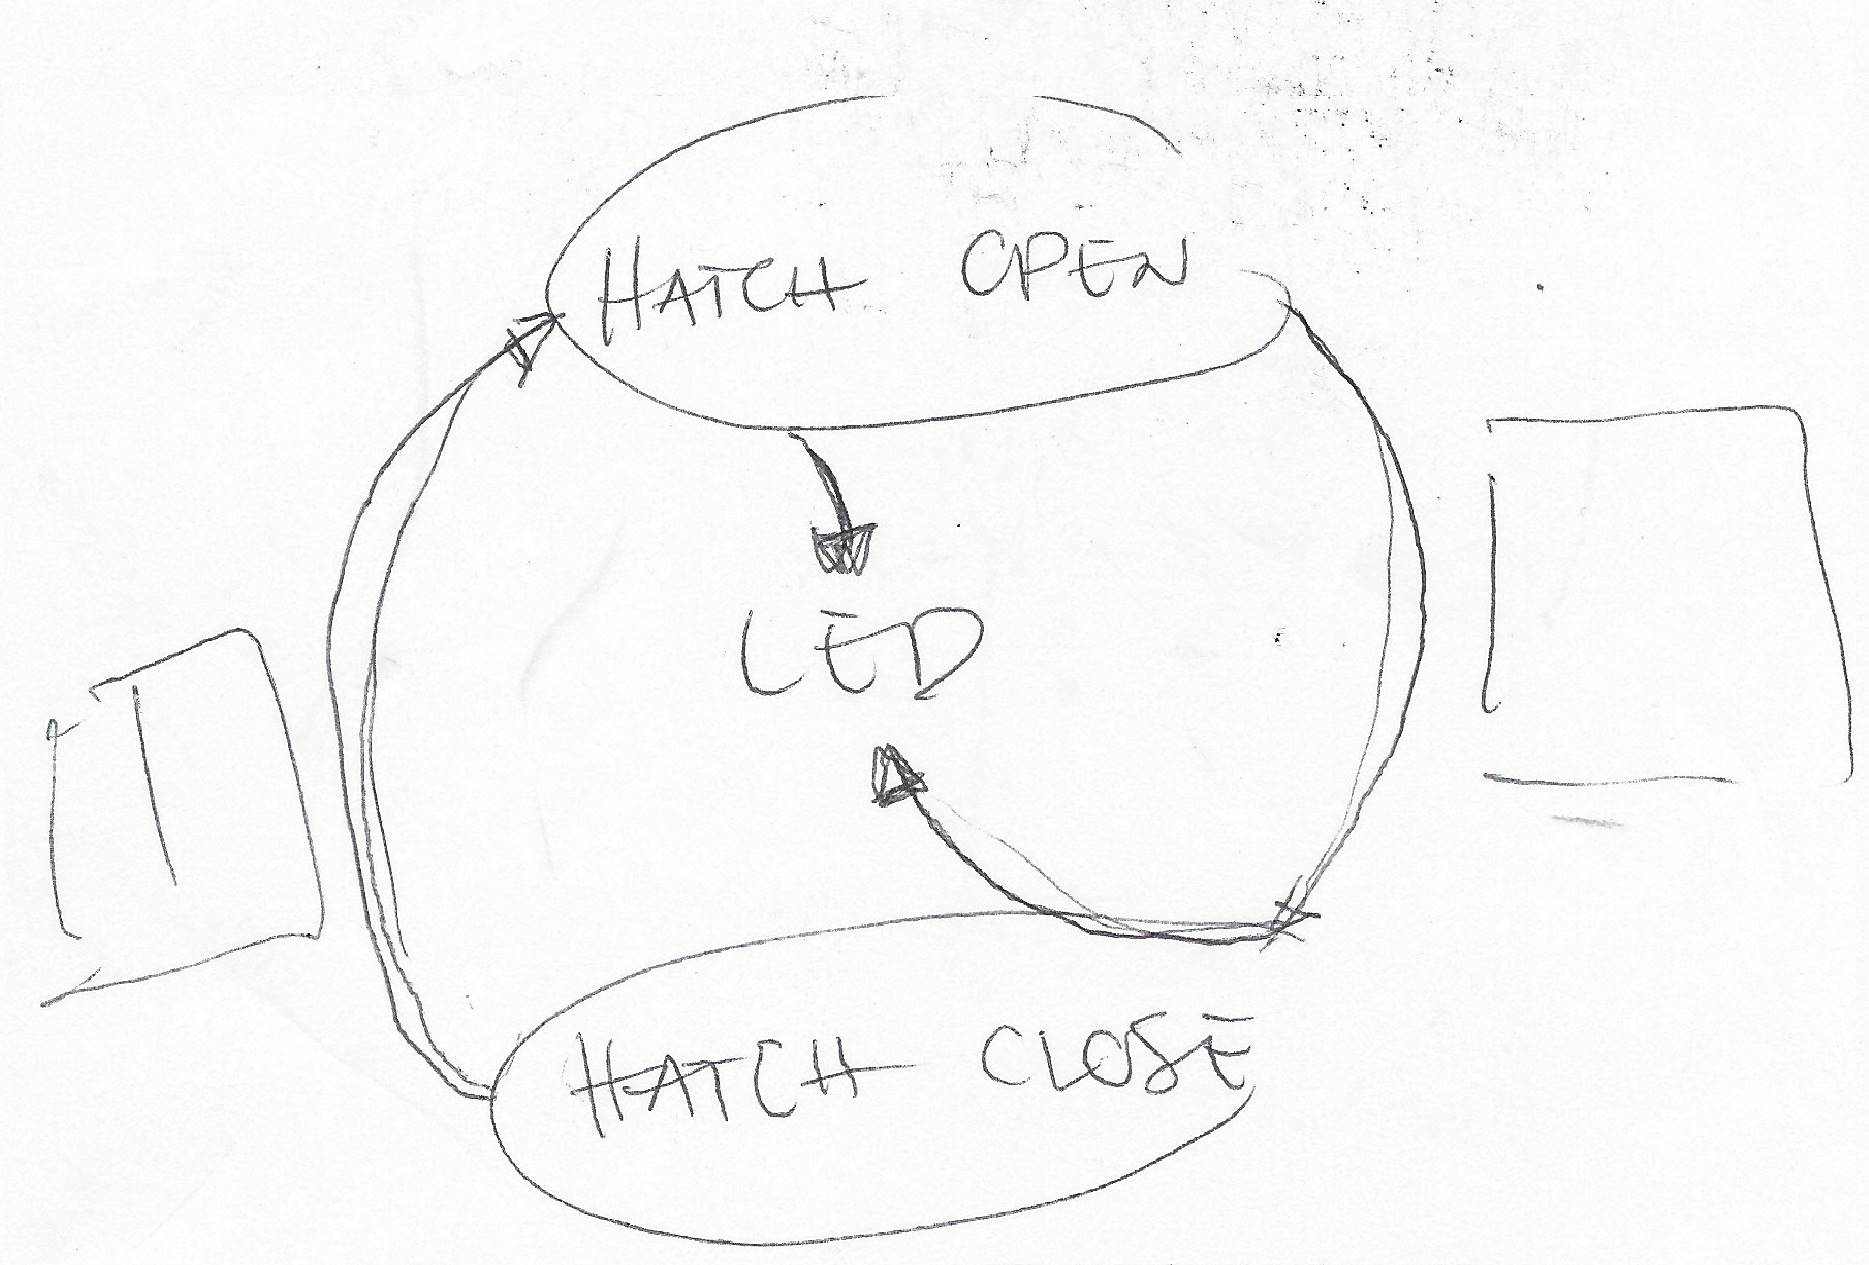
\includegraphics[width=.7\textwidth]{bilder/chapter5/joanna.jpg}
    \caption{Skizze eines Probanden, zur Erläuterung des mentalen Modells der Aktorsteuerung. Zu sehen ist, dass die Zustände in denen sich der Aktor befindet (''\textit{Hatch Open}'', etc.) Einfluss haben auf die zukünftige modifizierung der Aktoreigenschaften (hier: ''\textit{LED}'').  Dies ist prinzipiell identisch zum Konzeptmodell von flowws, welches die Übergänge zwischen den Zuständen nutzt, um die Eigenschaften zu modifzieren.}
    \label{fig:enduserskizze}
\end{figure}

Die Probanden konnten aus eigener Kraft oder nach kurzer Herleitung, innerhalb der ca. 30 minütigen Interviews sich die grundsätzlichen Prinzipien soweit aneignen, dass sie die Verhalten der Graphen antizipieren konnten. Eine der Probanden zeichnete eine Skizze (siehe Abbildung \ref{fig:enduserskizze}), wie sie die Steuerung des LED-Aktors (\hyperref[szenario2]{Szenario \#3}) verstanden hat. Die Skizze zeigt, dass die Programmatik der \ac{FSM} verstanden wurde und die Diskrepanzen zwischen Konzept- und mentalem Modell zur Steuerung von Aktoren überwindbar sind. Der Datenfluss selbst, stellte sich als grundsätzlich intuitiv für Probanden mit wenig Vorkenntnissen heraus. Es werden allerdings noch weitere Verbesserungen hinsichtlich Darstellung und Animationen benötigt, um das Zusammenspiel zwischen Datenfluss und \ac{FSM} zu verdeutlichen.

Leider konnten die Fit-Kriterien der nichtfunktionalen Anforderungen und somit Ziele (siehe Kapitel \ref{sec:1_zielsetzung}), aufgrund zeitlicher Beschränkungen, nicht vollständig erfüllt bzw. überprüft werden. Trotzdem wird flowws als einen ersten Erfolg gewertet, indem es eine innovatives \ac{EUD}-Werkzeug konzipiert, welches flexibel genug ist, um die Komplexität von \ac{IoT}-Prototypen abzubilden, aber nicht zu komplex ist, als dass es einen unzumutbaren Lernaufwand besitzt.  

Es steht außer Frage, dass noch zusätzliche Nutzertests mit weiterentwickelten Prototypen und einer größeren Anzahl von Probanden durchgeführt werden müssen, um ein umfassendes Bild darüber zu erhalten, ob flowws als \ac{EUD}-Werkzeug zum Prototyping produktiv eingesetzt werden kann.